% automatically generated document using lt2circuiTikz
\documentclass[tikz,margin={2pt 2pt 2pt 2pt}]{standalone}
\usepackage[compatibility,siunitx,  americanvoltages, americancurrents, americanresistors, europeaninductors, americanports,%
  straightlabels, fetbodydiode, straightvoltages]{circuitikz}
\usepackage{tikz,amsmath, amssymb,bm,color,pgfkeys,siunitx,ifthen,ulem}
\usepackage{pgfplots}
\pgfplotsset{compat=1.14}
\usetikzlibrary{shapes,arrows}
%\usepackage{agaramondc}					% Adobe Garamond, custom shape
%\renewcommand{\shapedefault}{rtl} % rtl: roman tabular lining

\makeatletter

%% bandstop filter (adapted from highpass)
\pgfcircdeclarebipole{}{\ctikzvalof{bipoles/highpass/width}}{*bandstop}{\ctikzvalof{bipoles/highpass/width}}{\ctikzvalof{bipoles/highpass/width}}{
	\pgf@circ@res@step = \ctikzvalof{bipoles/highpass/width}\pgf@circ@Rlen
	\divide \pgf@circ@res@step by 2
	
	\pgfpathmoveto{\pgfpoint{\pgf@circ@res@left}{\pgf@circ@res@zero}}
	\pgf@circ@res@other = \pgf@circ@res@left
	\advance\pgf@circ@res@other by \pgf@circ@res@step 
	
	\ifpgf@circuit@dashed
	\pgfsetdash{{0.1cm}{0.1cm}}{0cm} 
	\fi	
	
	% draw outer box
	\pgfsetlinewidth{\pgfkeysvalueof{/tikz/circuitikz/bipoles/thickness}\pgfstartlinewidth}
	\pgfpathrectanglecorners{\pgfpoint{\pgf@circ@res@left}{\pgf@circ@res@up}}{\pgfpoint{\pgf@circ@res@right}{\pgf@circ@res@down}}
	\pgfusepath{draw}
	
	\ifpgf@circuit@inputarrow
	{
		\advance \pgf@circ@res@left by -.5\pgfkeysvalueof{/tikz/circuitikz/bipoles/thickness}\pgfstartlinewidth
		\pgftransformshift{\pgfpoint{\pgf@circ@res@left}{0pt}}
		\pgfnode{inputarrow}{tip}{}{pgf@inputarrow}{\pgfusepath{fill}}
	}
	\fi
	
	% rotate inner symbol
	\def\pgfcircmathresult{\expandafter\pgf@circ@stripdecimals\pgf@circ@direction\pgf@nil}
	\ifnum \pgfcircmathresult > 45 \ifnum \pgfcircmathresult < 135
	\pgftransformrotate{270}
	\fi\fi
	\ifnum \pgfcircmathresult > 134 \ifnum \pgfcircmathresult < 225  % 134 degree, because >= 135 is not possible
	\pgftransformrotate{180}
	\fi\fi
	\ifnum \pgfcircmathresult > 224 \ifnum \pgfcircmathresult < 315
	\pgftransformrotate{90}
	\fi\fi
	
	% draw inner symbol
	\pgfsetdash{}{0pt}	% always draw solid line for inner symbol
	\pgfsetarrows{-} %never draw arrows
	\pgfsetlinewidth{\pgfstartlinewidth}
	\pgfpathmoveto{\pgfpoint{-0.5\pgf@circ@res@step}{0.5\pgf@circ@res@step}}
	\pgfpathsine{\pgfpoint{.25\pgf@circ@res@step}{.25\pgf@circ@res@step}}
	\pgfpathcosine{\pgfpoint{.25\pgf@circ@res@step}{-.25\pgf@circ@res@step}}
	\pgfpathsine{\pgfpoint{.25\pgf@circ@res@step}{-.25\pgf@circ@res@step}}
	\pgfpathcosine{\pgfpoint{.25\pgf@circ@res@step}{.25\pgf@circ@res@step}}
	\pgfusepath{draw}
	
	\pgfpathmoveto{\pgfpoint{-0.5\pgf@circ@res@step}{0}}
	\pgfpathsine{\pgfpoint{.25\pgf@circ@res@step}{.25\pgf@circ@res@step}}
	\pgfpathcosine{\pgfpoint{.25\pgf@circ@res@step}{-.25\pgf@circ@res@step}}
	\pgfpathsine{\pgfpoint{.25\pgf@circ@res@step}{-.25\pgf@circ@res@step}}
	\pgfpathcosine{\pgfpoint{.25\pgf@circ@res@step}{.25\pgf@circ@res@step}}
	\pgfusepath{draw}
	\pgfpathmoveto{\pgfpoint{-0.15\pgf@circ@res@step}{-0.15\pgf@circ@res@step}}
	\pgfpathlineto{\pgfpoint{0.15\pgf@circ@res@step}{0.15\pgf@circ@res@step}}
	\pgfusepath{draw}
	
	\pgfpathmoveto{\pgfpoint{-0.5\pgf@circ@res@step}{-0.5\pgf@circ@res@step}}
	\pgfpathsine{\pgfpoint{.25\pgf@circ@res@step}{.25\pgf@circ@res@step}}
	\pgfpathcosine{\pgfpoint{.25\pgf@circ@res@step}{-.25\pgf@circ@res@step}}
	\pgfpathsine{\pgfpoint{.25\pgf@circ@res@step}{-.25\pgf@circ@res@step}}
	\pgfpathcosine{\pgfpoint{.25\pgf@circ@res@step}{.25\pgf@circ@res@step}}
	\pgfusepath{draw}
	%	\pgfpathmoveto{\pgfpoint{-0.15\pgf@circ@res@step}{-0.65\pgf@circ@res@step}}
	%	\pgfpathlineto{\pgfpoint{0.15\pgf@circ@res@step}{-0.35\pgf@circ@res@step}}
	%	\pgfusepath{draw}
}

\tikzset{
	*bandstop/.style={\circuitikzbasekey, /tikz/to path=\pgf@circ@*bandstop@path},
}
\def\pgf@circ@*bandstop@path#1{\pgf@circ@bipole@path{*bandstop}{#1}}




\makeatother

\usetikzlibrary{backgrounds,calc,positioning}

\usetikzlibrary{circuits.ee.IEC}
\usetikzlibrary{arrows}


% sym32a style

\ctikzset{tripoles/mos style/arrows}
\ctikzset{
	/tikz/circuitikz/quadpoles/coupler/width=1,%1.3
	/tikz/circuitikz/quadpoles/coupler/height=0.952,%1.3
	/tikz/circuitikz/quadpoles/coupler2/width=1,%1.3
	/tikz/circuitikz/quadpoles/coupler2/height=0.952,%1.3
	/tikz/circuitikz/quadpoles/transformer/width=1.425,%1.5
	/tikz/circuitikz/quadpoles/transformer/height=1.425,%1.5
	/tikz/circuitikz/quadpoles/transformer core/width=1.425,%1.5
	/tikz/circuitikz/quadpoles/transformer core/height=1.425,%1.5
	/tikz/circuitikz/quadpoles/gyrator/width=1.425,%1.5
	/tikz/circuitikz/quadpoles/gyrator/height=1.425,%1.5
	%/tikz/circuitikz/monopoles/tlinestub/width=0.1875,%0.25 no effect!
	/tikz/circuitikz/tripoles/american and port/height=0.95,%.8
	/tikz/circuitikz/tripoles/american nand port/height=0.95,%.8
	/tikz/circuitikz/tripoles/american or port/height=0.95,%.8
	/tikz/circuitikz/tripoles/american nor port/height=0.95,%.8
	/tikz/circuitikz/tripoles/american xor port/height=0.95,%.8
	/tikz/circuitikz/tripoles/american xnor port/height=0.95,%.8
	/tikz/circuitikz/bipoles/tline/height=0.4,%0.3
%	/tikz/circuitikz/bipoles/tline/width=1.2,%0.8
	/tikz/circuitikz/bipoles/diode/height=0.375,%
	/tikz/circuitikz/bipoles/diode/width=0.375,%
	/tikz/circuitikz/bipoles/varcap/height=0.375,%
	/tikz/circuitikz/bipoles/varcap/width=0.375,%
	/tikz/circuitikz/tripoles/triac/height=1.05,%
	/tikz/circuitikz/tripoles/triac/width=0.952,%
	/tikz/circuitikz/tripoles/thyristor/height=1.05,%
	/tikz/circuitikz/tripoles/thyristor/width=0.952,%
	/tikz/circuitikz/tripoles/op amp/height=0.952,%
	/tikz/circuitikz/tripoles/op amp/width=1.2,%
	/tikz/circuitikz/tripoles/op amp/font=\footnotesize,
	/tikz/circuitikz/tripoles/gm amp/height=0.952,% 1.7
	/tikz/circuitikz/tripoles/gm amp/width=1.2,% 1.4
	%	/tikz/circuitikz/tripoles/gm amp/font=\footnotesize,
	/tikz/circuitikz/tripoles/plain amp/height=0.952,% 1.7
	/tikz/circuitikz/tripoles/plain amp/width=1.2,% 1.4
	/tikz/circuitikz/bipoles/resistor/voltage/straight label distance/.initial=.8,
	/tikz/circuitikz/bipoles/generic/voltage/straight label distance/.initial=.8,
	/tikz/circuitikz/bipoles/inductor/voltage/straight label distance/.initial=.8,
	/tikz/circuitikz/bipoles/fullgeneric/voltage/straight label distance/.initial=.8,
	/tikz/circuitikz/bipoles/capacitor/voltage/straight label distance/.initial=1.0,
	/tikz/circuitikz/bipoles/thickness=1.6,
}
\ctikzset{v/.append style={/tikz/european voltages}}

\definecolor{netlabelcolor}{rgb}{0, 0, 0.25}
\definecolor{lttotitextcolor}{rgb}{0, 0.4, 0.25}
\definecolor{lttotidrawcolor}{rgb}{0.6, 0.6, 0.6}
\definecolor{netcolor}{rgb}{0, 0, 0.5}

\pgfkeys{/lt2ti/netlabel/font/.initial= \small}
\pgfkeys{/lt2ti/text/font/.initial= \small}

\pgfkeys{/lt2ti/Net/.style= {netcolor}}
\tikzstyle{dashdotdotted}=[dash pattern=on 3pt off 2pt on \the\pgflinewidth off 2pt on \the\pgflinewidth off 2pt]

\pgfkeys{/lt2ti/VArrow/.style= {->,>=latex}}
\pgfkeys{/lt2ti/SArrow/.style= {->,>=angle 90}}

\begin{document}%
	%\centering%
		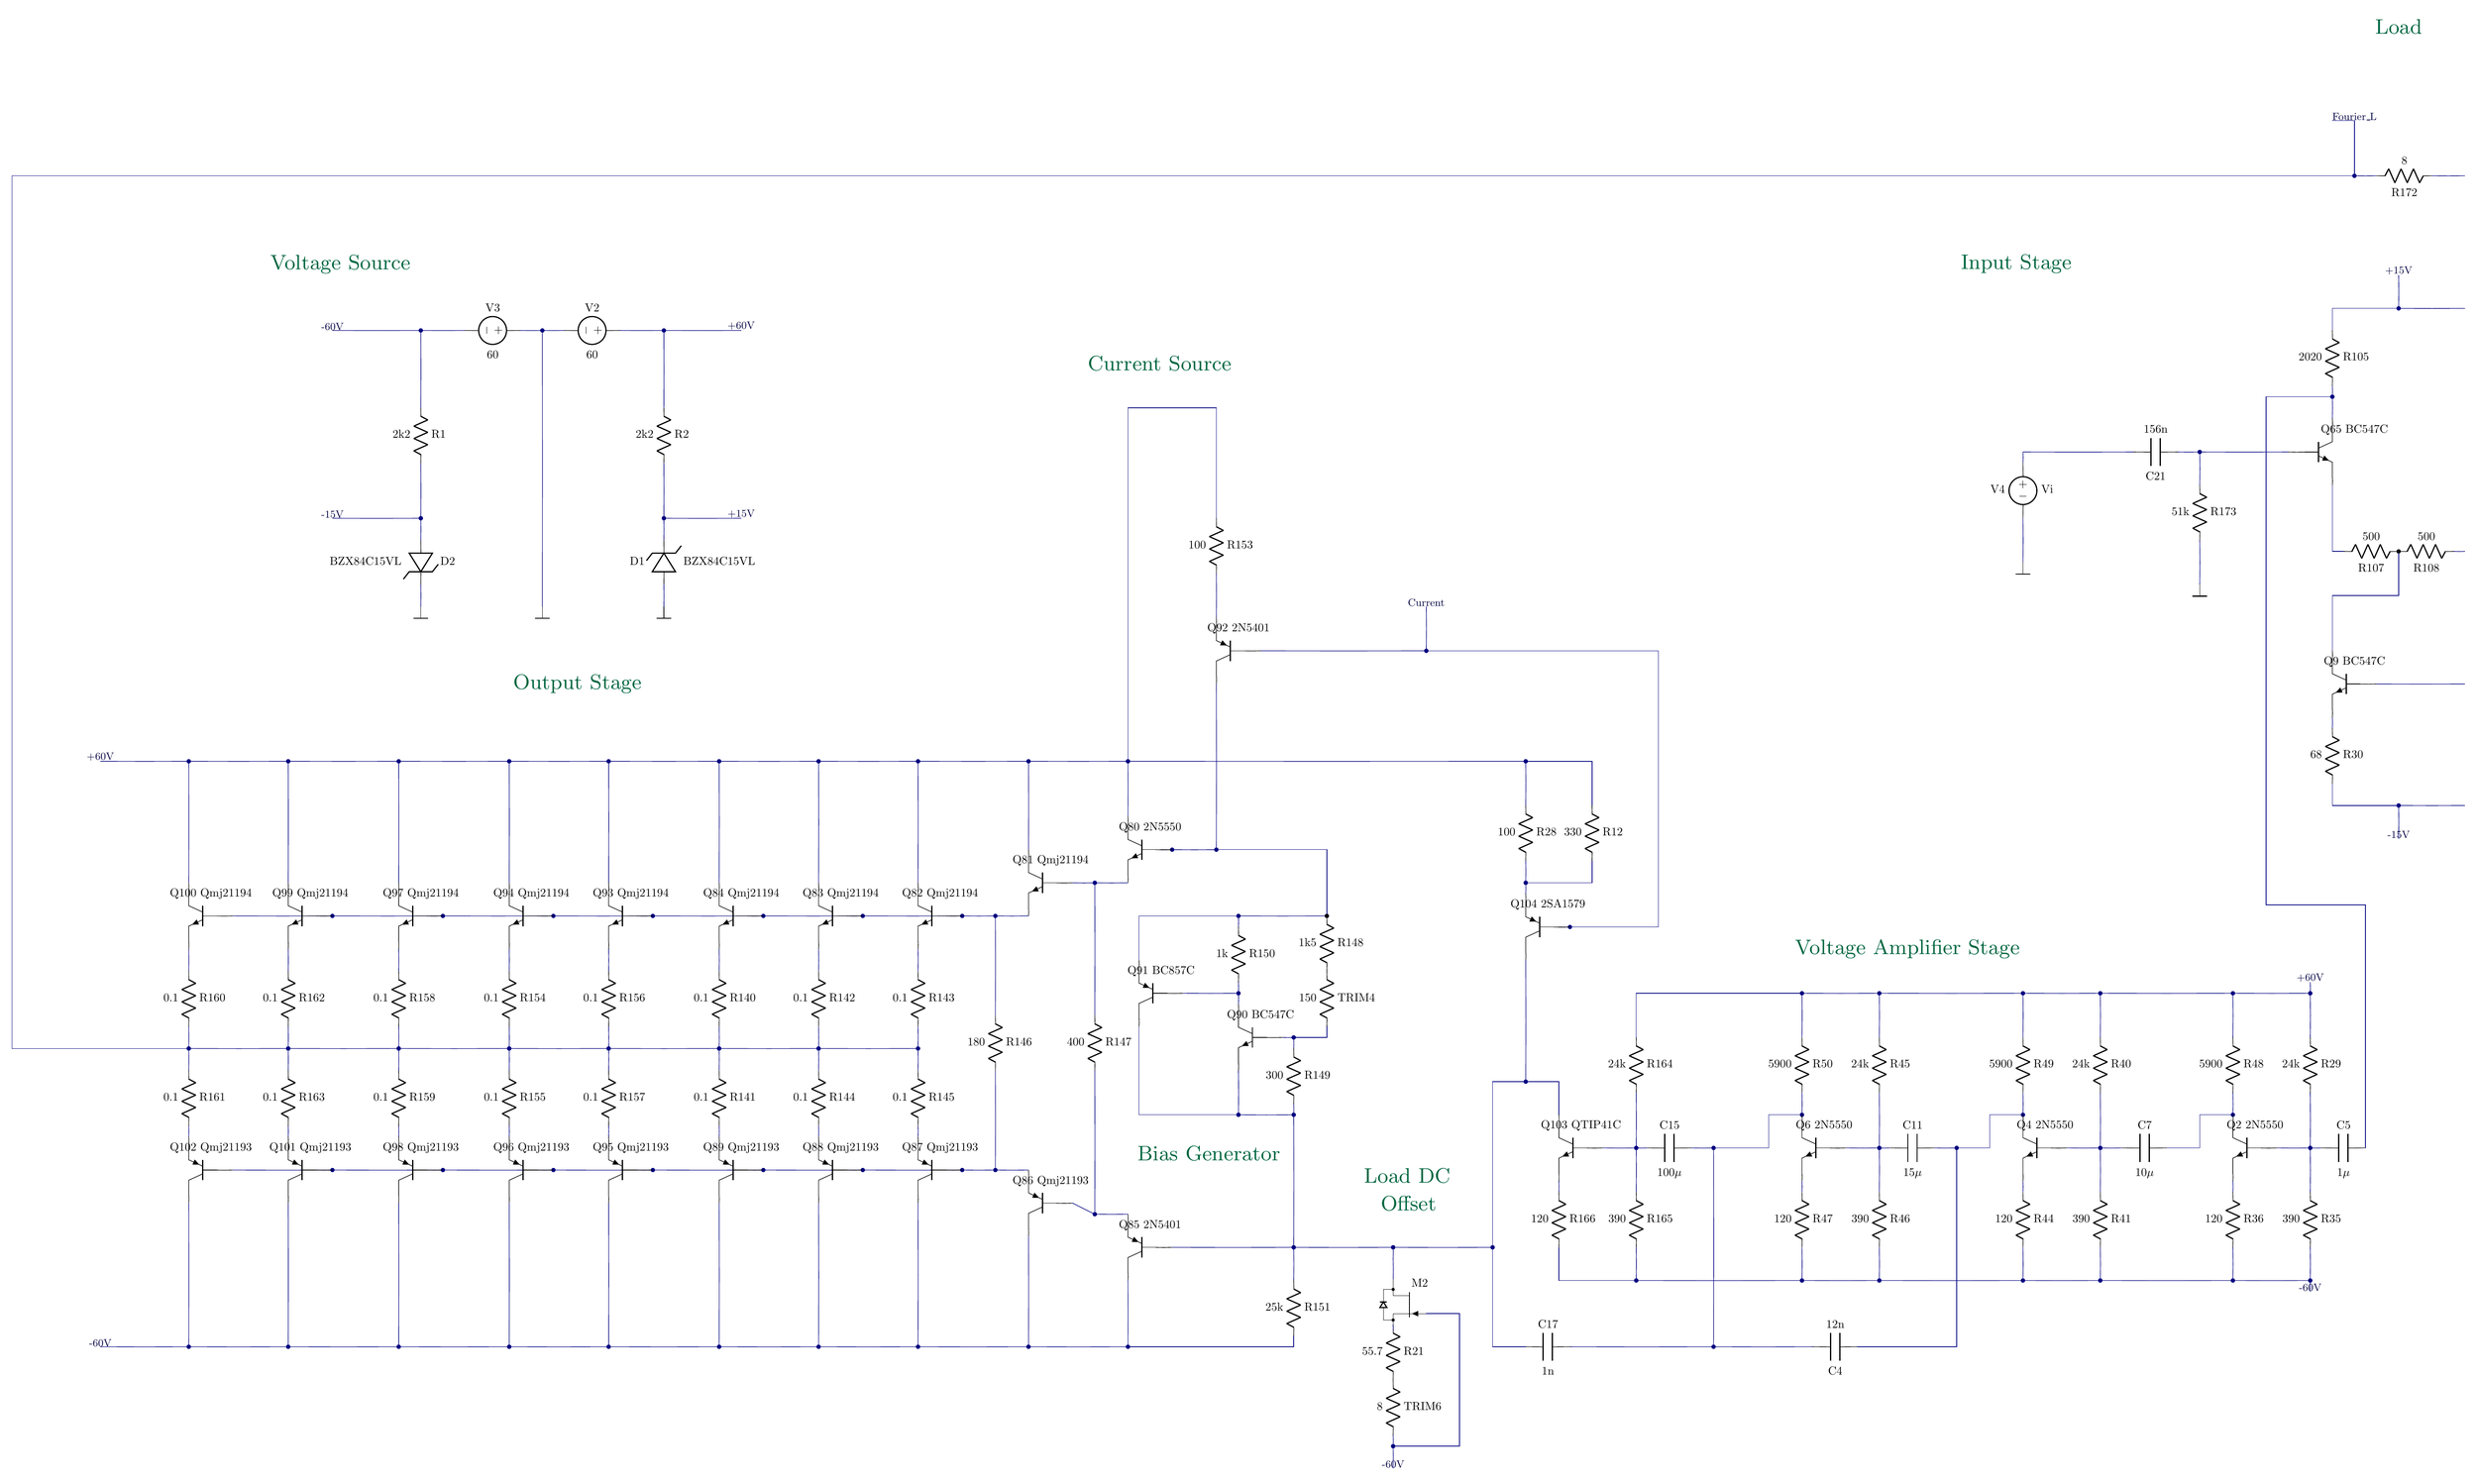
\begin{tikzpicture}[circuit ee IEC, scale=0.6666666667,line width=.5pt]% default: 0.4
	%\tikzstyle{every node}=[font=\small];%
	%\node [draw] at (0.0,0.0) {\pgfkeysvalueof{/tikz/circuitikz/tripoles/op amp/font}};
\draw [/lt2ti/Net](240.5,-131.5)to[*short,*-, color=netcolor] (240.5,-131.5);% wire w3_w4 start
\draw [/lt2ti/Net](239.5,-129.0)to[*short,-, color=netcolor] (239.5,-129.0);% wire w3_w4 end
\draw [/lt2ti/Net](240.5,-131.5) --  (240.5,-129.0) -- (239.5,-129.0); % wire w3_w4 polyline 
\draw [/lt2ti/Net](241.5,-131.5)to[*short,-*, color=netcolor] (240.5,-131.5);% wire w6
\draw [/lt2ti/Net](245.5,-131.5)to[*short,-, color=netcolor] (244.0,-131.5);% wire w7
\draw [/lt2ti/Net](242.5,-137.5)to[*short,*-, color=netcolor] (242.5,-136.0);% wire w8
\draw [/lt2ti/Net](242.5,-137.5)to[*short,*-, color=netcolor] (242.5,-137.5);% wire w9_w17 start
\draw [/lt2ti/Net](239.5,-138.5)to[*short,-, color=netcolor] (239.5,-138.5);% wire w9_w17 end
\draw [/lt2ti/Net](242.5,-137.5) --  (239.5,-137.5) -- (239.5,-138.5); % wire w9_w17 polyline 
\draw [/lt2ti/Net](245.5,-137.5)to[*short,-*, color=netcolor] (242.5,-137.5);% wire w10
\draw [/lt2ti/Net](153.0,-138.5)to[*short,*-, color=netcolor] (149.0,-138.5);% wire w11
\draw [/lt2ti/Net](155.0,-138.5)to[*short,-*, color=netcolor] (153.0,-138.5);% wire w12
\draw [/lt2ti/Net](158.5,-138.5)to[*short,*-, color=netcolor] (157.5,-138.5);% wire w13
\draw [/lt2ti/Net](159.5,-138.5)to[*short,-*, color=netcolor] (158.5,-138.5);% wire w14
\draw [/lt2ti/Net](164.0,-138.5)to[*short,*-, color=netcolor] (162.0,-138.5);% wire w15
\draw [/lt2ti/Net](167.5,-138.5)to[*short,-*, color=netcolor] (164.0,-138.5);% wire w16
\draw [/lt2ti/Net](239.5,-141.5)to[*short,*-, color=netcolor] (239.5,-141.0);% wire w18
\draw [/lt2ti/Net](153.0,-142.0)to[*short,-*, color=netcolor] (153.0,-138.5);% wire w20
\draw [/lt2ti/Net](164.0,-142.0)to[*short,-*, color=netcolor] (164.0,-138.5);% wire w21
\draw [/lt2ti/Net](239.5,-142.5)to[*short,-*, color=netcolor] (239.5,-141.5);% wire w23
\draw [/lt2ti/Net](230.5,-144.0)to[*short,-, color=netcolor] (225.5,-144.0);% wire w24
\draw [/lt2ti/Net](233.5,-144.0)to[*short,*-, color=netcolor] (232.5,-144.0);% wire w25
\draw [/lt2ti/Net](237.5,-144.0)to[*short,-*, color=netcolor] (233.5,-144.0);% wire w26
\draw [/lt2ti/Net](225.5,-144.5)to[*short,-, color=netcolor] (225.5,-144.0);% wire w27
\draw [/lt2ti/Net](233.5,-145.5)to[*short,-*, color=netcolor] (233.5,-144.0);% wire w28
\draw [/lt2ti/Net](153.0,-147.0)to[*short,*-, color=netcolor] (153.0,-144.5);% wire w29
\draw [/lt2ti/Net](153.0,-147.0)to[*short,*-, color=netcolor] (149.0,-147.0);% wire w30
\draw [/lt2ti/Net](164.0,-147.0)to[*short,*-, color=netcolor] (164.0,-144.5);% wire w31
\draw [/lt2ti/Net](167.5,-147.0)to[*short,-*, color=netcolor] (164.0,-147.0);% wire w32
\draw [/lt2ti/Net](153.0,-148.0)to[*short,-*, color=netcolor] (153.0,-147.0);% wire w34
\draw [/lt2ti/Net](164.0,-148.0)to[*short,-*, color=netcolor] (164.0,-147.0);% wire w35
\draw [/lt2ti/Net](240.0,-148.5)to[*short,-, color=netcolor] (240.0,-148.5);% wire w36_w37 start
\draw [/lt2ti/Net](239.5,-145.5)to[*short,-, color=netcolor] (239.5,-145.5);% wire w36_w37 end
\draw [/lt2ti/Net](240.0,-148.5) --  (239.5,-148.5) -- (239.5,-145.5); % wire w36_w37 polyline 
\draw [/lt2ti/Net](245.5,-148.5)to[*short,-, color=netcolor] (245.0,-148.5);% wire w38
\draw [/lt2ti/Net](225.5,-149.0)to[*short,-, color=netcolor] (225.5,-147.0);% wire w39
\draw [/lt2ti/Net](233.5,-150.0)to[*short,-, color=netcolor] (233.5,-148.0);% wire w40
\draw [/lt2ti/Net](153.0,-151.0)to[*short,-, color=netcolor] (153.0,-150.0);% wire w43
\draw [/lt2ti/Net](158.5,-151.0)to[*short,-*, color=netcolor] (158.5,-138.5);% wire w44
\draw [/lt2ti/Net](164.0,-151.0)to[*short,-, color=netcolor] (164.0,-150.0);% wire w45
\draw [/lt2ti/Net](189.0,-151.5)to[*short,-, color=netcolor] (189.0,-149.5);% wire w46
\draw [/lt2ti/Net](198.5,-153.0)to[*short,*-, color=netcolor] (198.5,-151.0);% wire w47
\draw [/lt2ti/Net](198.5,-153.0)to[*short,*-, color=netcolor] (191.0,-153.0);% wire w48
\draw [/lt2ti/Net](239.5,-153.0)to[*short,-, color=netcolor] (239.5,-153.0);% wire w50_w41_w42 start
\draw [/lt2ti/Net](242.5,-148.5)to[*short,-*, color=netcolor] (242.5,-148.5);% wire w50_w41_w42 end
\draw [/lt2ti/Net](239.5,-153.0) --  (239.5,-150.5) --  (242.5,-150.5) -- (242.5,-148.5); % wire w50_w41_w42 polyline 
\draw [/lt2ti/Net](245.5,-154.5)to[*short,-, color=netcolor] (241.5,-154.5);% wire w51
\draw [/lt2ti/Net](239.5,-156.5)to[*short,-, color=netcolor] (239.5,-156.0);% wire w52
\draw [/lt2ti/Net](142.5,-158.0)to[*short,*-, color=netcolor] (138.5,-158.0);% wire w53
\draw [/lt2ti/Net](147.0,-158.0)to[*short,*-*, color=netcolor] (142.5,-158.0);% wire w54
\draw [/lt2ti/Net](152.0,-158.0)to[*short,*-*, color=netcolor] (147.0,-158.0);% wire w55
\draw [/lt2ti/Net](157.0,-158.0)to[*short,*-*, color=netcolor] (152.0,-158.0);% wire w56
\draw [/lt2ti/Net](161.5,-158.0)to[*short,*-*, color=netcolor] (157.0,-158.0);% wire w57
\draw [/lt2ti/Net](166.5,-158.0)to[*short,*-*, color=netcolor] (161.5,-158.0);% wire w58
\draw [/lt2ti/Net](171.0,-158.0)to[*short,*-*, color=netcolor] (166.5,-158.0);% wire w59
\draw [/lt2ti/Net](175.5,-158.0)to[*short,*-*, color=netcolor] (171.0,-158.0);% wire w60
\draw [/lt2ti/Net](180.5,-158.0)to[*short,*-*, color=netcolor] (175.5,-158.0);% wire w61
\draw [/lt2ti/Net](185.0,-158.0)to[*short,*-*, color=netcolor] (180.5,-158.0);% wire w63
\draw [/lt2ti/Net](185.0,-158.0)to[*short,*-, color=netcolor] (185.0,-158.0);% wire w62_w22_w33 start
\draw [/lt2ti/Net](189.0,-147.0)to[*short,-, color=netcolor] (189.0,-147.0);% wire w62_w22_w33 end
\draw [/lt2ti/Net](185.0,-158.0) --  (185.0,-142.0) --  (189.0,-142.0) -- (189.0,-147.0); % wire w62_w22_w33 polyline 
\draw [/lt2ti/Net](203.0,-158.0)to[*short,*-*, color=netcolor] (185.0,-158.0);% wire w64
\draw [/lt2ti/Net](203.0,-160.0)to[*short,-*, color=netcolor] (203.0,-158.0);% wire w66
\draw [/lt2ti/Net](206.0,-160.0)to[*short,-, color=netcolor] (206.0,-160.0);% wire w65_w67 start
\draw [/lt2ti/Net](203.0,-158.0)to[*short,-*, color=netcolor] (203.0,-158.0);% wire w65_w67 end
\draw [/lt2ti/Net](206.0,-160.0) --  (206.0,-158.0) -- (203.0,-158.0); % wire w65_w67 polyline 
\draw [/lt2ti/Net](242.5,-160.0)to[*short,*-, color=netcolor] (242.5,-160.0);% wire w68_w69 start
\draw [/lt2ti/Net](239.5,-159.0)to[*short,-, color=netcolor] (239.5,-159.0);% wire w68_w69 end
\draw [/lt2ti/Net](242.5,-160.0) --  (239.5,-160.0) -- (239.5,-159.0); % wire w68_w69 polyline 
\draw [/lt2ti/Net](245.5,-160.0)to[*short,-*, color=netcolor] (242.5,-160.0);% wire w70
\draw [/lt2ti/Net](185.0,-160.5)to[*short,-*, color=netcolor] (185.0,-158.0);% wire w71
\draw [/lt2ti/Net](242.5,-161.5)to[*short,-*, color=netcolor] (242.5,-160.0);% wire w72
\draw [/lt2ti/Net](180.5,-162.0)to[*short,-*, color=netcolor] (180.5,-158.0);% wire w73
\draw [/lt2ti/Net](187.0,-162.0)to[*short,*-, color=netcolor] (186.5,-162.0);% wire w74
\draw [/lt2ti/Net](189.0,-162.0)to[*short,*-, color=netcolor] (189.0,-154.5);% wire w75
\draw [/lt2ti/Net](189.0,-162.0)to[*short,*-*, color=netcolor] (187.0,-162.0);% wire w76
\draw [/lt2ti/Net](142.5,-163.5)to[*short,-*, color=netcolor] (142.5,-158.0);% wire w78
\draw [/lt2ti/Net](147.0,-163.5)to[*short,-*, color=netcolor] (147.0,-158.0);% wire w79
\draw [/lt2ti/Net](152.0,-163.5)to[*short,-*, color=netcolor] (152.0,-158.0);% wire w80
\draw [/lt2ti/Net](157.0,-163.5)to[*short,-*, color=netcolor] (157.0,-158.0);% wire w81
\draw [/lt2ti/Net](161.5,-163.5)to[*short,-*, color=netcolor] (161.5,-158.0);% wire w82
\draw [/lt2ti/Net](166.5,-163.5)to[*short,-*, color=netcolor] (166.5,-158.0);% wire w83
\draw [/lt2ti/Net](171.0,-163.5)to[*short,-*, color=netcolor] (171.0,-158.0);% wire w84
\draw [/lt2ti/Net](175.5,-163.5)to[*short,-*, color=netcolor] (175.5,-158.0);% wire w85
\draw [/lt2ti/Net](183.5,-163.5)to[*short,*-, color=netcolor] (182.5,-163.5);% wire w86
\draw [/lt2ti/Net](185.0,-163.5)to[*short,-*, color=netcolor] (183.5,-163.5);% wire w87
\draw [/lt2ti/Net](203.0,-163.5)to[*short,*-, color=netcolor] (203.0,-162.5);% wire w88
\draw [/lt2ti/Net](206.0,-162.5)to[*short,-, color=netcolor] (206.0,-162.5);% wire w89_w90 start
\draw [/lt2ti/Net](203.0,-163.5)to[*short,-*, color=netcolor] (203.0,-163.5);% wire w89_w90 end
\draw [/lt2ti/Net](206.0,-162.5) --  (206.0,-163.5) -- (203.0,-163.5); % wire w89_w90 polyline 
\draw [/lt2ti/Net](203.0,-164.0)to[*short,-*, color=netcolor] (203.0,-163.5);% wire w91
\draw [/lt2ti/Net](149.0,-165.0)to[*short,*-, color=netcolor] (144.5,-165.0);% wire w94
\draw [/lt2ti/Net](154.0,-165.0)to[*short,*-*, color=netcolor] (149.0,-165.0);% wire w95
\draw [/lt2ti/Net](159.0,-165.0)to[*short,*-*, color=netcolor] (154.0,-165.0);% wire w96
\draw [/lt2ti/Net](163.5,-165.0)to[*short,*-*, color=netcolor] (159.0,-165.0);% wire w97
\draw [/lt2ti/Net](168.5,-165.0)to[*short,*-*, color=netcolor] (163.5,-165.0);% wire w98
\draw [/lt2ti/Net](173.0,-165.0)to[*short,*-*, color=netcolor] (168.5,-165.0);% wire w99
\draw [/lt2ti/Net](177.5,-165.0)to[*short,*-*, color=netcolor] (173.0,-165.0);% wire w100
\draw [/lt2ti/Net](179.0,-165.0)to[*short,*-*, color=netcolor] (177.5,-165.0);% wire w101
\draw [/lt2ti/Net](180.5,-165.0)to[*short,-*, color=netcolor] (179.0,-165.0);% wire w102
\draw [/lt2ti/Net](190.0,-165.0)to[*short,*-, color=netcolor] (190.0,-165.0);% wire w103_w110 start
\draw [/lt2ti/Net](185.5,-167.0)to[*short,-, color=netcolor] (185.5,-167.0);% wire w103_w110 end
\draw [/lt2ti/Net](190.0,-165.0) --  (185.5,-165.0) -- (185.5,-167.0); % wire w103_w110 polyline 
\draw [/lt2ti/Net](194.0,-165.0)to[*short,*-*, color=netcolor] (190.0,-165.0);% wire w105
\draw [/lt2ti/Net](194.0,-165.0)to[*short,*-, color=netcolor] (194.0,-165.0);% wire w77_w104 start
\draw [/lt2ti/Net](189.0,-162.0)to[*short,-*, color=netcolor] (189.0,-162.0);% wire w77_w104 end
\draw [/lt2ti/Net](194.0,-165.0) --  (194.0,-162.0) -- (189.0,-162.0); % wire w77_w104 polyline 
\draw [/lt2ti/Net](190.0,-165.5)to[*short,-*, color=netcolor] (190.0,-165.0);% wire w106
\draw [/lt2ti/Net](205.0,-165.5)to[*short,*-, color=netcolor] (204.5,-165.5);% wire w107
\draw [/lt2ti/Net](205.0,-165.5)to[*short,*-, color=netcolor] (205.0,-165.5);% wire w109_w49_w108 start
\draw [/lt2ti/Net](198.5,-153.0)to[*short,-*, color=netcolor] (198.5,-153.0);% wire w109_w49_w108 end
\draw [/lt2ti/Net](205.0,-165.5) --  (209.0,-165.5) --  (209.0,-153.0) -- (198.5,-153.0); % wire w109_w49_w108 polyline 
\draw [/lt2ti/Net](142.5,-167.5)to[*short,-, color=netcolor] (142.5,-166.5);% wire w111
\draw [/lt2ti/Net](147.0,-167.5)to[*short,-, color=netcolor] (147.0,-166.5);% wire w112
\draw [/lt2ti/Net](152.0,-167.5)to[*short,-, color=netcolor] (152.0,-166.5);% wire w113
\draw [/lt2ti/Net](157.0,-167.5)to[*short,-, color=netcolor] (157.0,-166.5);% wire w114
\draw [/lt2ti/Net](161.5,-167.5)to[*short,-, color=netcolor] (161.5,-166.5);% wire w115
\draw [/lt2ti/Net](166.5,-167.5)to[*short,-, color=netcolor] (166.5,-166.5);% wire w116
\draw [/lt2ti/Net](171.0,-167.5)to[*short,-, color=netcolor] (171.0,-166.5);% wire w117
\draw [/lt2ti/Net](175.5,-167.5)to[*short,-, color=netcolor] (175.5,-166.5);% wire w118
\draw [/lt2ti/Net](190.0,-168.5)to[*short,*-, color=netcolor] (190.0,-168.0);% wire w119
\draw [/lt2ti/Net](190.0,-168.5)to[*short,*-, color=netcolor] (187.5,-168.5);% wire w120
\draw [/lt2ti/Net](215.5,-168.5)to[*short,*-, color=netcolor] (215.5,-168.5);% wire w121_w134 start
\draw [/lt2ti/Net](208.0,-170.5)to[*short,-, color=netcolor] (208.0,-170.5);% wire w121_w134 end
\draw [/lt2ti/Net](215.5,-168.5) --  (208.0,-168.5) -- (208.0,-170.5); % wire w121_w134 polyline 
\draw [/lt2ti/Net](219.0,-168.5)to[*short,*-*, color=netcolor] (215.5,-168.5);% wire w122
\draw [/lt2ti/Net](225.5,-168.5)to[*short,*-*, color=netcolor] (219.0,-168.5);% wire w123
\draw [/lt2ti/Net](229.0,-168.5)to[*short,*-*, color=netcolor] (225.5,-168.5);% wire w124
\draw [/lt2ti/Net](235.0,-168.5)to[*short,*-*, color=netcolor] (229.0,-168.5);% wire w125
\draw [/lt2ti/Net](238.5,-168.5)to[*short,*-, color=netcolor] (238.5,-168.0);% wire w126
\draw [/lt2ti/Net](238.5,-168.5)to[*short,*-*, color=netcolor] (235.0,-168.5);% wire w127
\draw [/lt2ti/Net](190.0,-169.0)to[*short,-*, color=netcolor] (190.0,-168.5);% wire w128
\draw [/lt2ti/Net](179.0,-169.5)to[*short,-*, color=netcolor] (179.0,-165.0);% wire w129
\draw [/lt2ti/Net](183.5,-169.5)to[*short,-*, color=netcolor] (183.5,-163.5);% wire w130
\draw [/lt2ti/Net](192.5,-170.5)to[*short,*-, color=netcolor] (192.0,-170.5);% wire w131
\draw [/lt2ti/Net](194.0,-170.0)to[*short,-, color=netcolor] (194.0,-170.0);% wire w132_w133 start
\draw [/lt2ti/Net](192.5,-170.5)to[*short,-*, color=netcolor] (192.5,-170.5);% wire w132_w133 end
\draw [/lt2ti/Net](194.0,-170.0) --  (194.0,-170.5) -- (192.5,-170.5); % wire w132_w133 polyline 
\draw [/lt2ti/Net](215.5,-170.5)to[*short,-*, color=netcolor] (215.5,-168.5);% wire w135
\draw [/lt2ti/Net](219.0,-170.5)to[*short,-*, color=netcolor] (219.0,-168.5);% wire w136
\draw [/lt2ti/Net](225.5,-170.5)to[*short,-*, color=netcolor] (225.5,-168.5);% wire w137
\draw [/lt2ti/Net](229.0,-170.5)to[*short,-*, color=netcolor] (229.0,-168.5);% wire w138
\draw [/lt2ti/Net](235.0,-170.5)to[*short,-*, color=netcolor] (235.0,-168.5);% wire w139
\draw [/lt2ti/Net](238.5,-170.5)to[*short,-*, color=netcolor] (238.5,-168.5);% wire w140
\draw [/lt2ti/Net](142.5,-171.0)to[*short,*-, color=netcolor] (142.5,-170.0);% wire w142
\draw [/lt2ti/Net](142.5,-171.0)to[*short,*-, color=netcolor] (142.5,-171.0);% wire w143_w5_w141 start
\draw [/lt2ti/Net](240.5,-131.5)to[*short,-*, color=netcolor] (240.5,-131.5);% wire w143_w5_w141 end
\draw [/lt2ti/Net](142.5,-171.0) --  (134.5,-171.0) --  (134.5,-131.5) -- (240.5,-131.5); % wire w143_w5_w141 polyline 
\draw [/lt2ti/Net](147.0,-171.0)to[*short,*-, color=netcolor] (147.0,-170.0);% wire w144
\draw [/lt2ti/Net](147.0,-171.0)to[*short,*-*, color=netcolor] (142.5,-171.0);% wire w145
\draw [/lt2ti/Net](152.0,-171.0)to[*short,*-, color=netcolor] (152.0,-170.0);% wire w146
\draw [/lt2ti/Net](152.0,-171.0)to[*short,*-*, color=netcolor] (147.0,-171.0);% wire w147
\draw [/lt2ti/Net](157.0,-171.0)to[*short,*-, color=netcolor] (157.0,-170.0);% wire w148
\draw [/lt2ti/Net](157.0,-171.0)to[*short,*-*, color=netcolor] (152.0,-171.0);% wire w149
\draw [/lt2ti/Net](161.5,-171.0)to[*short,*-, color=netcolor] (161.5,-170.0);% wire w150
\draw [/lt2ti/Net](161.5,-171.0)to[*short,*-*, color=netcolor] (157.0,-171.0);% wire w151
\draw [/lt2ti/Net](166.5,-171.0)to[*short,*-, color=netcolor] (166.5,-170.0);% wire w152
\draw [/lt2ti/Net](166.5,-171.0)to[*short,*-*, color=netcolor] (161.5,-171.0);% wire w153
\draw [/lt2ti/Net](171.0,-171.0)to[*short,*-, color=netcolor] (171.0,-170.0);% wire w154
\draw [/lt2ti/Net](171.0,-171.0)to[*short,*-*, color=netcolor] (166.5,-171.0);% wire w155
\draw [/lt2ti/Net](175.5,-171.0)to[*short,*-, color=netcolor] (175.5,-170.0);% wire w156
\draw [/lt2ti/Net](175.5,-171.0)to[*short,*-*, color=netcolor] (171.0,-171.0);% wire w157
\draw [/lt2ti/Net](192.5,-171.0)to[*short,-*, color=netcolor] (192.5,-170.5);% wire w158
\draw [/lt2ti/Net](142.5,-172.0)to[*short,-*, color=netcolor] (142.5,-171.0);% wire w159
\draw [/lt2ti/Net](147.0,-172.0)to[*short,-*, color=netcolor] (147.0,-171.0);% wire w160
\draw [/lt2ti/Net](152.0,-172.0)to[*short,-*, color=netcolor] (152.0,-171.0);% wire w161
\draw [/lt2ti/Net](157.0,-172.0)to[*short,-*, color=netcolor] (157.0,-171.0);% wire w162
\draw [/lt2ti/Net](161.5,-172.0)to[*short,-*, color=netcolor] (161.5,-171.0);% wire w163
\draw [/lt2ti/Net](166.5,-172.0)to[*short,-*, color=netcolor] (166.5,-171.0);% wire w164
\draw [/lt2ti/Net](171.0,-172.0)to[*short,-*, color=netcolor] (171.0,-171.0);% wire w165
\draw [/lt2ti/Net](175.5,-172.0)to[*short,-*, color=netcolor] (175.5,-171.0);% wire w166
\draw [/lt2ti/Net](203.0,-172.5)to[*short,*-, color=netcolor] (203.0,-167.0);% wire w167
\draw [/lt2ti/Net](203.0,-172.5)to[*short,*-, color=netcolor] (203.0,-172.5);% wire w168_w235 start
\draw [/lt2ti/Net](201.5,-180.0)to[*short,-*, color=netcolor] (201.5,-180.0);% wire w168_w235 end
\draw [/lt2ti/Net](203.0,-172.5) --  (201.5,-172.5) -- (201.5,-180.0); % wire w168_w235 polyline 
\draw [/lt2ti/Net](190.0,-174.0)to[*short,*-, color=netcolor] (190.0,-172.0);% wire w171
\draw [/lt2ti/Net](190.0,-174.0)to[*short,*-, color=netcolor] (190.0,-174.0);% wire w170_w172 start
\draw [/lt2ti/Net](185.5,-170.0)to[*short,-, color=netcolor] (185.5,-170.0);% wire w170_w172 end
\draw [/lt2ti/Net](190.0,-174.0) --  (185.5,-174.0) -- (185.5,-170.0); % wire w170_w172 polyline 
\draw [/lt2ti/Net](192.5,-174.0)to[*short,*-, color=netcolor] (192.5,-173.5);% wire w173
\draw [/lt2ti/Net](192.5,-174.0)to[*short,*-*, color=netcolor] (190.0,-174.0);% wire w174
\draw [/lt2ti/Net](204.5,-174.0)to[*short,-, color=netcolor] (204.5,-174.0);% wire w169_w175 start
\draw [/lt2ti/Net](203.0,-172.5)to[*short,-*, color=netcolor] (203.0,-172.5);% wire w169_w175 end
\draw [/lt2ti/Net](204.5,-174.0) --  (204.5,-172.5) -- (203.0,-172.5); % wire w169_w175 polyline 
\draw [/lt2ti/Net](215.5,-174.0)to[*short,*-, color=netcolor] (215.5,-173.0);% wire w176
\draw [/lt2ti/Net](215.5,-174.0)to[*short,*-, color=netcolor] (215.5,-174.0);% wire w195_w177_w194 start
\draw [/lt2ti/Net](211.5,-175.5)to[*short,-*, color=netcolor] (211.5,-175.5);% wire w195_w177_w194 end
\draw [/lt2ti/Net](215.5,-174.0) --  (214.0,-174.0) --  (214.0,-175.5) -- (211.5,-175.5); % wire w195_w177_w194 polyline 
\draw [/lt2ti/Net](225.5,-174.0)to[*short,*-, color=netcolor] (225.5,-173.0);% wire w178
\draw [/lt2ti/Net](225.5,-174.0)to[*short,*-, color=netcolor] (225.5,-174.0);% wire w201_w179_w200 start
\draw [/lt2ti/Net](222.5,-175.5)to[*short,-*, color=netcolor] (222.5,-175.5);% wire w201_w179_w200 end
\draw [/lt2ti/Net](225.5,-174.0) --  (224.0,-174.0) --  (224.0,-175.5) -- (222.5,-175.5); % wire w201_w179_w200 polyline 
\draw [/lt2ti/Net](235.0,-174.0)to[*short,*-, color=netcolor] (235.0,-173.0);% wire w180
\draw [/lt2ti/Net](235.0,-174.0)to[*short,*-, color=netcolor] (235.0,-174.0);% wire w206_w181_w205 start
\draw [/lt2ti/Net](232.0,-175.5)to[*short,-, color=netcolor] (232.0,-175.5);% wire w206_w181_w205 end
\draw [/lt2ti/Net](235.0,-174.0) --  (233.5,-174.0) --  (233.5,-175.5) -- (232.0,-175.5); % wire w206_w181_w205 polyline 
\draw [/lt2ti/Net](142.5,-175.0)to[*short,-, color=netcolor] (142.5,-174.5);% wire w182
\draw [/lt2ti/Net](147.0,-175.0)to[*short,-, color=netcolor] (147.0,-174.5);% wire w183
\draw [/lt2ti/Net](152.0,-175.0)to[*short,-, color=netcolor] (152.0,-174.5);% wire w184
\draw [/lt2ti/Net](157.0,-175.0)to[*short,-, color=netcolor] (157.0,-174.5);% wire w185
\draw [/lt2ti/Net](161.5,-175.0)to[*short,-, color=netcolor] (161.5,-174.5);% wire w186
\draw [/lt2ti/Net](166.5,-175.0)to[*short,-, color=netcolor] (166.5,-174.5);% wire w187
\draw [/lt2ti/Net](171.0,-175.0)to[*short,-, color=netcolor] (171.0,-174.5);% wire w188
\draw [/lt2ti/Net](175.5,-175.0)to[*short,-, color=netcolor] (175.5,-174.5);% wire w189
\draw [/lt2ti/Net](208.0,-175.5)to[*short,*-, color=netcolor] (208.0,-173.0);% wire w190
\draw [/lt2ti/Net](208.0,-175.5)to[*short,*-, color=netcolor] (206.5,-175.5);% wire w191
\draw [/lt2ti/Net](208.5,-175.5)to[*short,-*, color=netcolor] (208.0,-175.5);% wire w192
\draw [/lt2ti/Net](211.5,-175.5)to[*short,*-, color=netcolor] (210.5,-175.5);% wire w193
\draw [/lt2ti/Net](219.0,-175.5)to[*short,*-, color=netcolor] (219.0,-173.0);% wire w196
\draw [/lt2ti/Net](219.0,-175.5)to[*short,*-, color=netcolor] (217.5,-175.5);% wire w197
\draw [/lt2ti/Net](219.5,-175.5)to[*short,-*, color=netcolor] (219.0,-175.5);% wire w198
\draw [/lt2ti/Net](222.5,-175.5)to[*short,*-, color=netcolor] (221.5,-175.5);% wire w199
\draw [/lt2ti/Net](222.5,-175.5)to[*short,*-, color=netcolor] (222.5,-175.5);% wire w283_w284 start
\draw [/lt2ti/Net](218.0,-184.5)to[*short,-, color=netcolor] (218.0,-184.5);% wire w283_w284 end
\draw [/lt2ti/Net](222.5,-175.5) --  (222.5,-184.5) -- (218.0,-184.5); % wire w283_w284 polyline 
\draw [/lt2ti/Net](229.0,-175.5)to[*short,*-, color=netcolor] (229.0,-173.0);% wire w202
\draw [/lt2ti/Net](229.0,-175.5)to[*short,*-, color=netcolor] (227.5,-175.5);% wire w203
\draw [/lt2ti/Net](230.0,-175.5)to[*short,-*, color=netcolor] (229.0,-175.5);% wire w204
\draw [/lt2ti/Net](238.5,-175.5)to[*short,*-, color=netcolor] (238.5,-173.0);% wire w207
\draw [/lt2ti/Net](238.5,-175.5)to[*short,*-, color=netcolor] (237.0,-175.5);% wire w208
\draw [/lt2ti/Net](239.0,-175.5)to[*short,-*, color=netcolor] (238.5,-175.5);% wire w209
\draw [/lt2ti/Net](241.0,-175.5)to[*short,-, color=netcolor] (241.0,-175.5);% wire w210_w93_w19_w92 start
\draw [/lt2ti/Net](239.5,-141.5)to[*short,-*, color=netcolor] (239.5,-141.5);% wire w210_w93_w19_w92 end
\draw [/lt2ti/Net](241.0,-175.5) --  (241.0,-164.5) --  (236.5,-164.5) --  (236.5,-141.5) -- (239.5,-141.5); % wire w210_w93_w19_w92 polyline 
\draw [/lt2ti/Net](149.0,-176.5)to[*short,*-, color=netcolor] (144.5,-176.5);% wire w211
\draw [/lt2ti/Net](154.0,-176.5)to[*short,*-*, color=netcolor] (149.0,-176.5);% wire w212
\draw [/lt2ti/Net](159.0,-176.5)to[*short,*-*, color=netcolor] (154.0,-176.5);% wire w213
\draw [/lt2ti/Net](163.5,-176.5)to[*short,*-*, color=netcolor] (159.0,-176.5);% wire w214
\draw [/lt2ti/Net](168.5,-176.5)to[*short,*-*, color=netcolor] (163.5,-176.5);% wire w215
\draw [/lt2ti/Net](173.0,-176.5)to[*short,*-*, color=netcolor] (168.5,-176.5);% wire w216
\draw [/lt2ti/Net](177.5,-176.5)to[*short,*-*, color=netcolor] (173.0,-176.5);% wire w217
\draw [/lt2ti/Net](179.0,-176.5)to[*short,*-, color=netcolor] (179.0,-172.0);% wire w218
\draw [/lt2ti/Net](179.0,-176.5)to[*short,*-*, color=netcolor] (177.5,-176.5);% wire w219
\draw [/lt2ti/Net](180.5,-176.5)to[*short,-*, color=netcolor] (179.0,-176.5);% wire w220
\draw [/lt2ti/Net](204.5,-177.5)to[*short,-, color=netcolor] (204.5,-177.0);% wire w221
\draw [/lt2ti/Net](208.0,-177.5)to[*short,-*, color=netcolor] (208.0,-175.5);% wire w222
\draw [/lt2ti/Net](215.5,-177.5)to[*short,-, color=netcolor] (215.5,-177.0);% wire w223
\draw [/lt2ti/Net](219.0,-177.5)to[*short,-*, color=netcolor] (219.0,-175.5);% wire w224
\draw [/lt2ti/Net](225.5,-177.5)to[*short,-, color=netcolor] (225.5,-177.0);% wire w225
\draw [/lt2ti/Net](229.0,-177.5)to[*short,-*, color=netcolor] (229.0,-175.5);% wire w226
\draw [/lt2ti/Net](235.0,-177.5)to[*short,-, color=netcolor] (235.0,-177.0);% wire w227
\draw [/lt2ti/Net](238.5,-177.5)to[*short,-*, color=netcolor] (238.5,-175.5);% wire w228
\draw [/lt2ti/Net](183.5,-178.5)to[*short,*-, color=netcolor] (183.5,-172.0);% wire w229
\draw [/lt2ti/Net](183.5,-178.5)to[*short,*-, color=netcolor] (182.5,-178.0);% wire w230
\draw [/lt2ti/Net](185.0,-178.5)to[*short,-*, color=netcolor] (183.5,-178.5);% wire w231
\draw [/lt2ti/Net](192.5,-180.0)to[*short,*-*, color=netcolor] (192.5,-174.0);% wire w232
\draw [/lt2ti/Net](192.5,-180.0)to[*short,*-, color=netcolor] (187.0,-180.0);% wire w233
\draw [/lt2ti/Net](197.0,-180.0)to[*short,*-*, color=netcolor] (192.5,-180.0);% wire w234
\draw [/lt2ti/Net](201.5,-180.0)to[*short,*-*, color=netcolor] (197.0,-180.0);% wire w236
\draw [/lt2ti/Net](197.0,-180.5)to[*short,-*, color=netcolor] (197.0,-180.0);% wire w237
\draw [/lt2ti/Net](192.5,-181.5)to[*short,-*, color=netcolor] (192.5,-180.0);% wire w238
\draw [/lt2ti/Net](208.0,-181.5)to[*short,*-, color=netcolor] (208.0,-180.0);% wire w240
\draw [/lt2ti/Net](208.0,-181.5)to[*short,*-, color=netcolor] (208.0,-181.5);% wire w239_w241 start
\draw [/lt2ti/Net](204.5,-180.0)to[*short,-, color=netcolor] (204.5,-180.0);% wire w239_w241 end
\draw [/lt2ti/Net](208.0,-181.5) --  (204.5,-181.5) -- (204.5,-180.0); % wire w239_w241 polyline 
\draw [/lt2ti/Net](215.5,-181.5)to[*short,*-, color=netcolor] (215.5,-180.0);% wire w242
\draw [/lt2ti/Net](215.5,-181.5)to[*short,*-*, color=netcolor] (208.0,-181.5);% wire w243
\draw [/lt2ti/Net](219.0,-181.5)to[*short,*-, color=netcolor] (219.0,-180.0);% wire w244
\draw [/lt2ti/Net](219.0,-181.5)to[*short,*-*, color=netcolor] (215.5,-181.5);% wire w245
\draw [/lt2ti/Net](225.5,-181.5)to[*short,*-, color=netcolor] (225.5,-180.0);% wire w246
\draw [/lt2ti/Net](225.5,-181.5)to[*short,*-*, color=netcolor] (219.0,-181.5);% wire w247
\draw [/lt2ti/Net](229.0,-181.5)to[*short,*-, color=netcolor] (229.0,-180.0);% wire w248
\draw [/lt2ti/Net](229.0,-181.5)to[*short,*-*, color=netcolor] (225.5,-181.5);% wire w249
\draw [/lt2ti/Net](235.0,-181.5)to[*short,*-, color=netcolor] (235.0,-180.0);% wire w250
\draw [/lt2ti/Net](235.0,-181.5)to[*short,*-*, color=netcolor] (229.0,-181.5);% wire w251
\draw [/lt2ti/Net](238.5,-181.5)to[*short,*-, color=netcolor] (238.5,-180.0);% wire w252
\draw [/lt2ti/Net](238.5,-181.5)to[*short,*-*, color=netcolor] (235.0,-181.5);% wire w253
\draw [/lt2ti/Net](238.5,-182.0)to[*short,-*, color=netcolor] (238.5,-181.5);% wire w254
\draw [/lt2ti/Net](142.5,-184.5)to[*short,*-, color=netcolor] (142.5,-178.0);% wire w256
\draw [/lt2ti/Net](142.5,-184.5)to[*short,*-, color=netcolor] (138.5,-184.5);% wire w257
\draw [/lt2ti/Net](147.0,-184.5)to[*short,*-, color=netcolor] (147.0,-178.0);% wire w258
\draw [/lt2ti/Net](147.0,-184.5)to[*short,*-*, color=netcolor] (142.5,-184.5);% wire w259
\draw [/lt2ti/Net](152.0,-184.5)to[*short,*-, color=netcolor] (152.0,-178.0);% wire w260
\draw [/lt2ti/Net](152.0,-184.5)to[*short,*-*, color=netcolor] (147.0,-184.5);% wire w261
\draw [/lt2ti/Net](157.0,-184.5)to[*short,*-, color=netcolor] (157.0,-178.0);% wire w262
\draw [/lt2ti/Net](157.0,-184.5)to[*short,*-*, color=netcolor] (152.0,-184.5);% wire w263
\draw [/lt2ti/Net](161.5,-184.5)to[*short,*-, color=netcolor] (161.5,-178.0);% wire w264
\draw [/lt2ti/Net](161.5,-184.5)to[*short,*-*, color=netcolor] (157.0,-184.5);% wire w265
\draw [/lt2ti/Net](166.5,-184.5)to[*short,*-, color=netcolor] (166.5,-178.0);% wire w266
\draw [/lt2ti/Net](166.5,-184.5)to[*short,*-*, color=netcolor] (161.5,-184.5);% wire w267
\draw [/lt2ti/Net](171.0,-184.5)to[*short,*-, color=netcolor] (171.0,-178.0);% wire w268
\draw [/lt2ti/Net](171.0,-184.5)to[*short,*-*, color=netcolor] (166.5,-184.5);% wire w269
\draw [/lt2ti/Net](175.5,-184.5)to[*short,*-, color=netcolor] (175.5,-178.0);% wire w270
\draw [/lt2ti/Net](175.5,-184.5)to[*short,*-*, color=netcolor] (171.0,-184.5);% wire w271
\draw [/lt2ti/Net](180.5,-184.5)to[*short,*-, color=netcolor] (180.5,-179.5);% wire w272
\draw [/lt2ti/Net](180.5,-184.5)to[*short,*-*, color=netcolor] (175.5,-184.5);% wire w273
\draw [/lt2ti/Net](185.0,-184.5)to[*short,*-, color=netcolor] (185.0,-181.5);% wire w274
\draw [/lt2ti/Net](185.0,-184.5)to[*short,*-*, color=netcolor] (180.5,-184.5);% wire w275
\draw [/lt2ti/Net](192.5,-184.0)to[*short,-, color=netcolor] (192.5,-184.0);% wire w276_w277 start
\draw [/lt2ti/Net](185.0,-184.5)to[*short,-*, color=netcolor] (185.0,-184.5);% wire w276_w277 end
\draw [/lt2ti/Net](192.5,-184.0) --  (192.5,-184.5) -- (185.0,-184.5); % wire w276_w277 polyline 
\draw [/lt2ti/Net](203.0,-184.5)to[*short,-, color=netcolor] (203.0,-184.5);% wire w278_w279 start
\draw [/lt2ti/Net](201.5,-180.0)to[*short,-*, color=netcolor] (201.5,-180.0);% wire w278_w279 end
\draw [/lt2ti/Net](203.0,-184.5) --  (201.5,-184.5) -- (201.5,-180.0); % wire w278_w279 polyline 
\draw [/lt2ti/Net](211.5,-184.5)to[*short,*-*, color=netcolor] (211.5,-175.5);% wire w280
\draw [/lt2ti/Net](211.5,-184.5)to[*short,*-, color=netcolor] (205.0,-184.5);% wire w281
\draw [/lt2ti/Net](216.0,-184.5)to[*short,-*, color=netcolor] (211.5,-184.5);% wire w282
\draw [/lt2ti/Net](197.0,-189.0)to[*short,*-, color=netcolor] (197.0,-188.5);% wire w285
\draw [/lt2ti/Net](197.0,-189.0)to[*short,*-, color=netcolor] (197.0,-189.0);% wire w287_w255_w286 start
\draw [/lt2ti/Net](198.5,-183.0)to[*short,-, color=netcolor] (198.5,-183.0);% wire w287_w255_w286 end
\draw [/lt2ti/Net](197.0,-189.0) --  (200.0,-189.0) --  (200.0,-183.0) -- (198.5,-183.0); % wire w287_w255_w286 polyline 
\draw [/lt2ti/Net](197.0,-190.0)to[*short,-*, color=netcolor] (197.0,-189.0);% wire w288
 \draw (158.5, -151.0) node[rground, xscale=1, yscale=1, rotate=0, ] (undefined) {};%  (undefined)++(0.0,0.0) node {undefined }; % component "circuiTikz\gnd" "undefined" 
 \draw (225.5, -149.0) node[rground, xscale=1, yscale=1, rotate=0, ] (undefined) {};%  (undefined)++(0.0,0.0) node {undefined }; % component "circuiTikz\gnd" "undefined" 
 \draw (233.5, -150.0) node[rground, xscale=1, yscale=1, rotate=0, ] (undefined) {};%  (undefined)++(0.0,0.0) node {undefined }; % component "circuiTikz\gnd" "undefined" 
 \draw (164.0, -151.0) node[rground, xscale=1, yscale=1, rotate=0, ] (undefined) {};%  (undefined)++(0.0,0.0) node {undefined }; % component "circuiTikz\gnd" "undefined" 
 \draw (153.0, -151.0) node[rground, xscale=1, yscale=1, rotate=0, ] (undefined) {};%  (undefined)++(0.0,0.0) node {undefined }; % component "circuiTikz\gnd" "undefined" 
  \draw (162.0, -138.5) to[*V, l_=V2, a^=60,, -, ] (159.5,-138.5){}; % component "voltage" "V2" 
  \draw (157.5, -138.5) to[*V, l_=V3, a^=60,, -, ] (155.0,-138.5){}; % component "voltage" "V3" 
 \draw (239.5, -144.0) node[npn, nobodydiode, , rotate=0, ] (Q65) {}   (Q65)++(1.0,1) node {Q65 BC547C}; % component "npn" "Q65" 
 \draw (237.5, -144.0) to [*short, -] (Q65.B); \draw (239.5, -145.5) to [*short, -] (Q65.E); \draw (239.5, -142.5) to [*short, -] (Q65.C);% extend wires to the connection points   % component "npn" "Q65" 
  \draw (239.5, -138.5) to[*resistor, l^=R105, a_=2020, -, ] (239.5,-141.0){}; %\node [] at (239.0,-138.0) {x}; % component "res" "R105" 
  \draw (242.5, -148.5) to[*resistor, l^=R107, a_=500, *-, ] (240.0,-148.5){}; %\node [] at (243.0,-148.0) {x}; % component "res" "R107" 
  \draw (245.0, -148.5) to[*resistor, l^=R108, a_=500, -, ] (242.5,-148.5){}; %\node [] at (245.5,-148.0) {x}; % component "res" "R108" 
 \draw (185.0, -162.0) node[npn, nobodydiode, xscale=-1, rotate=0, ] (Q80) {}   (Q80)++(1.0,1) node {Q80 2N5550}; % component "npn" "Q80" 
 \draw (187.0, -162.0) to [*short, -] (Q80.B); \draw (185.0, -163.5) to [*short, -] (Q80.E); \draw (185.0, -160.5) to [*short, -] (Q80.C);% extend wires to the connection points   % component "npn" "Q80" 
 \draw (180.5, -163.5) node[npn, nobodydiode, xscale=-1, rotate=0, ] (Q81) {}   (Q81)++(1.0,1) node {Q81 Qmj21194}; % component "npn" "Q81" 
 \draw (182.5, -163.5) to [*short, -] (Q81.B); \draw (180.5, -165.0) to [*short, -] (Q81.E); \draw (180.5, -162.0) to [*short, -] (Q81.C);% extend wires to the connection points   % component "npn" "Q81" 
 \draw (175.5, -165.0) node[npn, nobodydiode, xscale=-1, rotate=0, ] (Q82) {}   (Q82)++(1.0,1) node {Q82 Qmj21194}; % component "npn" "Q82" 
 \draw (177.5, -165.0) to [*short, -] (Q82.B); \draw (175.5, -166.5) to [*short, -] (Q82.E); \draw (175.5, -163.5) to [*short, -] (Q82.C);% extend wires to the connection points   % component "npn" "Q82" 
 \draw (171.0, -165.0) node[npn, nobodydiode, xscale=-1, rotate=0, ] (Q83) {}   (Q83)++(1.0,1) node {Q83 Qmj21194}; % component "npn" "Q83" 
 \draw (173.0, -165.0) to [*short, -] (Q83.B); \draw (171.0, -166.5) to [*short, -] (Q83.E); \draw (171.0, -163.5) to [*short, -] (Q83.C);% extend wires to the connection points   % component "npn" "Q83" 
 \draw (166.5, -165.0) node[npn, nobodydiode, xscale=-1, rotate=0, ] (Q84) {}   (Q84)++(1.0,1) node {Q84 Qmj21194}; % component "npn" "Q84" 
 \draw (168.5, -165.0) to [*short, -] (Q84.B); \draw (166.5, -166.5) to [*short, -] (Q84.E); \draw (166.5, -163.5) to [*short, -] (Q84.C);% extend wires to the connection points   % component "npn" "Q84" 
 \draw (185.0, -180.0) node[pnp, nobodydiode, xscale=-1, yscale=1, rotate=-360, ] (Q85) {}   (Q85)++(1.0,1) node {Q85 2N5401}; % component "pnp" "Q85" 
 \draw (187.0, -180.0) to [*short, -] (Q85.B); \draw (185.0, -178.5) to [*short, -] (Q85.E); \draw (185.0, -181.5) to [*short, -] (Q85.C);% extend wires to the connection points   % component "pnp" "Q85" 
 \draw (180.5, -178.0) node[pnp, nobodydiode, xscale=-1, yscale=1, rotate=-360, ] (Q86) {}   (Q86)++(1.0,1) node {Q86 Qmj21193}; % component "pnp" "Q86" 
 \draw (182.5, -178.0) to [*short, -] (Q86.B); \draw (180.5, -176.5) to [*short, -] (Q86.E); \draw (180.5, -179.5) to [*short, -] (Q86.C);% extend wires to the connection points   % component "pnp" "Q86" 
 \draw (175.5, -176.5) node[pnp, nobodydiode, xscale=-1, yscale=1, rotate=-360, ] (Q87) {}   (Q87)++(1.0,1) node {Q87 Qmj21193}; % component "pnp" "Q87" 
 \draw (177.5, -176.5) to [*short, -] (Q87.B); \draw (175.5, -175.0) to [*short, -] (Q87.E); \draw (175.5, -178.0) to [*short, -] (Q87.C);% extend wires to the connection points   % component "pnp" "Q87" 
 \draw (171.0, -176.5) node[pnp, nobodydiode, xscale=-1, yscale=1, rotate=-360, ] (Q88) {}   (Q88)++(1.0,1) node {Q88 Qmj21193}; % component "pnp" "Q88" 
 \draw (173.0, -176.5) to [*short, -] (Q88.B); \draw (171.0, -175.0) to [*short, -] (Q88.E); \draw (171.0, -178.0) to [*short, -] (Q88.C);% extend wires to the connection points   % component "pnp" "Q88" 
 \draw (166.5, -176.5) node[pnp, nobodydiode, xscale=-1, yscale=1, rotate=-360, ] (Q89) {}   (Q89)++(1.0,1) node {Q89 Qmj21193}; % component "pnp" "Q89" 
 \draw (168.5, -176.5) to [*short, -] (Q89.B); \draw (166.5, -175.0) to [*short, -] (Q89.E); \draw (166.5, -178.0) to [*short, -] (Q89.C);% extend wires to the connection points   % component "pnp" "Q89" 
  \draw (166.5, -167.5) to[*resistor, l^=R140, a_=0.1, -, ] (166.5,-170.0){}; %\node [] at (167.0,-167.0) {x}; % component "res" "R140" 
  \draw (166.5, -172.0) to[*resistor, l^=R141, a_=0.1, -, ] (166.5,-174.5){}; %\node [] at (167.0,-171.5) {x}; % component "res" "R141" 
  \draw (171.0, -167.5) to[*resistor, l^=R142, a_=0.1, -, ] (171.0,-170.0){}; %\node [] at (171.5,-167.0) {x}; % component "res" "R142" 
  \draw (175.5, -167.5) to[*resistor, l^=R143, a_=0.1, -, ] (175.5,-170.0){}; %\node [] at (176.0,-167.0) {x}; % component "res" "R143" 
  \draw (171.0, -172.0) to[*resistor, l^=R144, a_=0.1, -, ] (171.0,-174.5){}; %\node [] at (171.5,-171.5) {x}; % component "res" "R144" 
  \draw (175.5, -172.0) to[*resistor, l^=R145, a_=0.1, -, ] (175.5,-174.5){}; %\node [] at (176.0,-171.5) {x}; % component "res" "R145" 
  \draw (179.0, -169.5) to[*resistor, l^=R146, a_=180, -, ] (179.0,-172.0){}; %\node [] at (179.5,-169.0) {x}; % component "res" "R146" 
  \draw (183.5, -169.5) to[*resistor, l^=R147, a_=400, -, ] (183.5,-172.0){}; %\node [] at (184.0,-169.0) {x}; % component "res" "R147" 
 \draw (190.0, -170.5) node[npn, nobodydiode, xscale=-1, rotate=0, ] (Q90) {}   (Q90)++(1.0,1) node {Q90 BC547C}; % component "npn" "Q90" 
 \draw (192.0, -170.5) to [*short, -] (Q90.B); \draw (190.0, -172.0) to [*short, -] (Q90.E); \draw (190.0, -169.0) to [*short, -] (Q90.C);% extend wires to the connection points   % component "npn" "Q90" 
  \draw (194.0, -165.0) to[*resistor, l^=R148, a_=1k5, *-, ] (194.0,-167.5){}; %\node [] at (194.5,-164.5) {x}; % component "res" "R148" 
  \draw (192.5, -171.0) to[*resistor, l^=R149, a_=300, -, ] (192.5,-173.5){}; %\node [] at (193.0,-170.5) {x}; % component "res" "R149" 
  \draw (190.0, -165.5) to[*resistor, l^=R150, a_=1k, -, ] (190.0,-168.0){}; %\node [] at (190.5,-165.0) {x}; % component "res" "R150" 
 \draw (185.5, -168.5) node[pnp, nobodydiode, xscale=-1, yscale=1, rotate=-360, ] (Q91) {}   (Q91)++(1.0,1) node {Q91 BC857C}; % component "pnp" "Q91" 
 \draw (187.5, -168.5) to [*short, -] (Q91.B); \draw (185.5, -167.0) to [*short, -] (Q91.E); \draw (185.5, -170.0) to [*short, -] (Q91.C);% extend wires to the connection points   % component "pnp" "Q91" 
  \draw (192.5, -181.5) to[*resistor, l^=R151, a_=25k, -, ] (192.5,-184.0){}; %\node [] at (193.0,-181.0) {x}; % component "res" "R151" 
 \draw (189.0, -153.0) node[pnp, nobodydiode, xscale=-1, yscale=1, rotate=-360, ] (Q92) {}   (Q92)++(1.0,1) node {Q92 2N5401}; % component "pnp" "Q92" 
 \draw (191.0, -153.0) to [*short, -] (Q92.B); \draw (189.0, -151.5) to [*short, -] (Q92.E); \draw (189.0, -154.5) to [*short, -] (Q92.C);% extend wires to the connection points   % component "pnp" "Q92" 
  \draw (189.0, -147.0) to[*resistor, l^=R153, a_=100, -, ] (189.0,-149.5){}; %\node [] at (189.5,-146.5) {x}; % component "res" "R153" 
 \draw (161.5, -165.0) node[npn, nobodydiode, xscale=-1, rotate=0, ] (Q93) {}   (Q93)++(1.0,1) node {Q93 Qmj21194}; % component "npn" "Q93" 
 \draw (163.5, -165.0) to [*short, -] (Q93.B); \draw (161.5, -166.5) to [*short, -] (Q93.E); \draw (161.5, -163.5) to [*short, -] (Q93.C);% extend wires to the connection points   % component "npn" "Q93" 
 \draw (157.0, -165.0) node[npn, nobodydiode, xscale=-1, rotate=0, ] (Q94) {}   (Q94)++(1.0,1) node {Q94 Qmj21194}; % component "npn" "Q94" 
 \draw (159.0, -165.0) to [*short, -] (Q94.B); \draw (157.0, -166.5) to [*short, -] (Q94.E); \draw (157.0, -163.5) to [*short, -] (Q94.C);% extend wires to the connection points   % component "npn" "Q94" 
 \draw (161.5, -176.5) node[pnp, nobodydiode, xscale=-1, yscale=1, rotate=-360, ] (Q95) {}   (Q95)++(1.0,1) node {Q95 Qmj21193}; % component "pnp" "Q95" 
 \draw (163.5, -176.5) to [*short, -] (Q95.B); \draw (161.5, -175.0) to [*short, -] (Q95.E); \draw (161.5, -178.0) to [*short, -] (Q95.C);% extend wires to the connection points   % component "pnp" "Q95" 
 \draw (157.0, -176.5) node[pnp, nobodydiode, xscale=-1, yscale=1, rotate=-360, ] (Q96) {}   (Q96)++(1.0,1) node {Q96 Qmj21193}; % component "pnp" "Q96" 
 \draw (159.0, -176.5) to [*short, -] (Q96.B); \draw (157.0, -175.0) to [*short, -] (Q96.E); \draw (157.0, -178.0) to [*short, -] (Q96.C);% extend wires to the connection points   % component "pnp" "Q96" 
  \draw (157.0, -167.5) to[*resistor, l^=R154, a_=0.1, -, ] (157.0,-170.0){}; %\node [] at (157.5,-167.0) {x}; % component "res" "R154" 
  \draw (157.0, -172.0) to[*resistor, l^=R155, a_=0.1, -, ] (157.0,-174.5){}; %\node [] at (157.5,-171.5) {x}; % component "res" "R155" 
  \draw (161.5, -167.5) to[*resistor, l^=R156, a_=0.1, -, ] (161.5,-170.0){}; %\node [] at (162.0,-167.0) {x}; % component "res" "R156" 
  \draw (161.5, -172.0) to[*resistor, l^=R157, a_=0.1, -, ] (161.5,-174.5){}; %\node [] at (162.0,-171.5) {x}; % component "res" "R157" 
 \draw (152.0, -165.0) node[npn, nobodydiode, xscale=-1, rotate=0, ] (Q97) {}   (Q97)++(1.0,1) node {Q97 Qmj21194}; % component "npn" "Q97" 
 \draw (154.0, -165.0) to [*short, -] (Q97.B); \draw (152.0, -166.5) to [*short, -] (Q97.E); \draw (152.0, -163.5) to [*short, -] (Q97.C);% extend wires to the connection points   % component "npn" "Q97" 
 \draw (152.0, -176.5) node[pnp, nobodydiode, xscale=-1, yscale=1, rotate=-360, ] (Q98) {}   (Q98)++(1.0,1) node {Q98 Qmj21193}; % component "pnp" "Q98" 
 \draw (154.0, -176.5) to [*short, -] (Q98.B); \draw (152.0, -175.0) to [*short, -] (Q98.E); \draw (152.0, -178.0) to [*short, -] (Q98.C);% extend wires to the connection points   % component "pnp" "Q98" 
  \draw (152.0, -167.5) to[*resistor, l^=R158, a_=0.1, -, ] (152.0,-170.0){}; %\node [] at (152.5,-167.0) {x}; % component "res" "R158" 
  \draw (152.0, -172.0) to[*resistor, l^=R159, a_=0.1, -, ] (152.0,-174.5){}; %\node [] at (152.5,-171.5) {x}; % component "res" "R159" 
 \draw (147.0, -165.0) node[npn, nobodydiode, xscale=-1, rotate=0, ] (Q99) {}   (Q99)++(1.0,1) node {Q99 Qmj21194}; % component "npn" "Q99" 
 \draw (149.0, -165.0) to [*short, -] (Q99.B); \draw (147.0, -166.5) to [*short, -] (Q99.E); \draw (147.0, -163.5) to [*short, -] (Q99.C);% extend wires to the connection points   % component "npn" "Q99" 
 \draw (142.5, -165.0) node[npn, nobodydiode, xscale=-1, rotate=0, ] (Q100) {}   (Q100)++(1.0,1) node {Q100 Qmj21194}; % component "npn" "Q100" 
 \draw (144.5, -165.0) to [*short, -] (Q100.B); \draw (142.5, -166.5) to [*short, -] (Q100.E); \draw (142.5, -163.5) to [*short, -] (Q100.C);% extend wires to the connection points   % component "npn" "Q100" 
 \draw (147.0, -176.5) node[pnp, nobodydiode, xscale=-1, yscale=1, rotate=-360, ] (Q101) {}   (Q101)++(1.0,1) node {Q101 Qmj21193}; % component "pnp" "Q101" 
 \draw (149.0, -176.5) to [*short, -] (Q101.B); \draw (147.0, -175.0) to [*short, -] (Q101.E); \draw (147.0, -178.0) to [*short, -] (Q101.C);% extend wires to the connection points   % component "pnp" "Q101" 
 \draw (142.5, -176.5) node[pnp, nobodydiode, xscale=-1, yscale=1, rotate=-360, ] (Q102) {}   (Q102)++(1.0,1) node {Q102 Qmj21193}; % component "pnp" "Q102" 
 \draw (144.5, -176.5) to [*short, -] (Q102.B); \draw (142.5, -175.0) to [*short, -] (Q102.E); \draw (142.5, -178.0) to [*short, -] (Q102.C);% extend wires to the connection points   % component "pnp" "Q102" 
  \draw (142.5, -167.5) to[*resistor, l^=R160, a_=0.1, -, ] (142.5,-170.0){}; %\node [] at (143.0,-167.0) {x}; % component "res" "R160" 
  \draw (142.5, -172.0) to[*resistor, l^=R161, a_=0.1, -, ] (142.5,-174.5){}; %\node [] at (143.0,-171.5) {x}; % component "res" "R161" 
  \draw (147.0, -167.5) to[*resistor, l^=R162, a_=0.1, -, ] (147.0,-170.0){}; %\node [] at (147.5,-167.0) {x}; % component "res" "R162" 
  \draw (147.0, -172.0) to[*resistor, l^=R163, a_=0.1, -, ] (147.0,-174.5){}; %\node [] at (147.5,-171.5) {x}; % component "res" "R163" 
  \draw (208.0, -170.5) to[*resistor, l^=R164, a_=24k, -, ] (208.0,-173.0){}; %\node [] at (208.5,-170.0) {x}; % component "res" "R164" 
  \draw (208.0, -177.5) to[*resistor, l^=R165, a_=390, -, ] (208.0,-180.0){}; %\node [] at (208.5,-177.0) {x}; % component "res" "R165" 
 \draw (204.5, -175.5) node[npn, nobodydiode, xscale=-1, rotate=0, ] (Q103) {}   (Q103)++(1.0,1) node {Q103 QTIP41C}; % component "npn" "Q103" 
 \draw (206.5, -175.5) to [*short, -] (Q103.B); \draw (204.5, -177.0) to [*short, -] (Q103.E); \draw (204.5, -174.0) to [*short, -] (Q103.C);% extend wires to the connection points   % component "npn" "Q103" 
  \draw (204.5, -177.5) to[*resistor, l^=R166, a_=120, -, ] (204.5,-180.0){}; %\node [] at (205.0,-177.0) {x}; % component "res" "R166" 
 \draw (203.0, -165.5) node[pnp, nobodydiode, xscale=-1, yscale=1, rotate=-360, ] (Q104) {}   (Q104)++(1.0,1) node {Q104 2SA1579}; % component "pnp" "Q104" 
 \draw (205.0, -165.5) to [*short, -] (Q104.B); \draw (203.0, -164.0) to [*short, -] (Q104.E); \draw (203.0, -167.0) to [*short, -] (Q104.C);% extend wires to the connection points   % component "pnp" "Q104" 
  \draw (203.0, -184.5) to[*capacitor, l^=C17, a_=1n, -, ] (205.0,-184.5){}; % component "cap" "C17" 
  %\node [] at (203.0,-184.0) {x}; % component "cap" "C17" 
  \draw (225.5, -144.5) to[*V, l_=V4, a^=Vi,, -, ] (225.5,-147.0){}; % component "voltage" "V4" 
  \draw (232.5, -144.0) to[*capacitor, l^=C21, a_=156n, -, ] (230.5,-144.0){}; % component "cap" "C21" 
  %\node [] at (232.5,-143.5) {x}; % component "cap" "C21" 
  \draw (233.5, -145.5) to[*resistor, l^=R173, a_=51k, -, ] (233.5,-148.0){}; %\node [] at (234.0,-145.0) {x}; % component "res" "R173" 
  \draw (244.0, -131.5) to[*resistor, l^=R172, a_=8, -, ] (241.5,-131.5){}; %\node [] at (244.5,-131.0) {x}; % component "res" "R172" 
  \draw (164.0, -150.0) to[*zzDo, l^=D1, a_=BZX84C15VL, ] (164.0,-148.0){}; % component "zener" "D1" 
 %\node [] at (163.5,-150.0) {x}; % component "zener" "D1" 
  \draw (153.0, -148.0) to[*zzDo, l^=D2, a_=BZX84C15VL, ] (153.0,-150.0){}; % component "zener" "D2" 
 %\node [] at (153.5,-148.0) {x}; % component "zener" "D2" 
 \draw (239.5, -154.5) node[npn, nobodydiode, xscale=-1, rotate=0, ] (Q9) {}   (Q9)++(1.0,1) node {Q9 BC547C}; % component "npn" "Q9" 
 \draw (241.5, -154.5) to [*short, -] (Q9.B); \draw (239.5, -156.0) to [*short, -] (Q9.E); \draw (239.5, -153.0) to [*short, -] (Q9.C);% extend wires to the connection points   % component "npn" "Q9" 
  \draw (239.5, -156.5) to[*resistor, l^=R30, a_=68, -, ] (239.5,-159.0){}; %\node [] at (239.0,-156.0) {x}; % component "res" "R30" 
  \draw (203.0, -160.0) to[*resistor, l^=R28, a_=100, -, ] (203.0,-162.5){}; %\node [] at (202.5,-159.5) {x}; % component "res" "R28" 
  \draw (208.5, -175.5) to[*capacitor, l^=C15, a_=100$\mu$, -, ] (210.5,-175.5){}; % component "cap" "C15" 
  %\node [] at (208.5,-175.0) {x}; % component "cap" "C15" 
  \draw (238.5, -170.5) to[*resistor, l^=R29, a_=24k, -, ] (238.5,-173.0){}; %\node [] at (239.0,-170.0) {x}; % component "res" "R29" 
  \draw (238.5, -177.5) to[*resistor, l^=R35, a_=390, -, ] (238.5,-180.0){}; %\node [] at (239.0,-177.0) {x}; % component "res" "R35" 
 \draw (235.0, -175.5) node[npn, nobodydiode, xscale=-1, rotate=0, ] (Q2) {}   (Q2)++(1.0,1) node {Q2 2N5550}; % component "npn" "Q2" 
 \draw (237.0, -175.5) to [*short, -] (Q2.B); \draw (235.0, -177.0) to [*short, -] (Q2.E); \draw (235.0, -174.0) to [*short, -] (Q2.C);% extend wires to the connection points   % component "npn" "Q2" 
  \draw (235.0, -177.5) to[*resistor, l^=R36, a_=120, -, ] (235.0,-180.0){}; %\node [] at (235.5,-177.0) {x}; % component "res" "R36" 
  \draw (229.0, -170.5) to[*resistor, l^=R40, a_=24k, -, ] (229.0,-173.0){}; %\node [] at (229.5,-170.0) {x}; % component "res" "R40" 
  \draw (229.0, -177.5) to[*resistor, l^=R41, a_=390, -, ] (229.0,-180.0){}; %\node [] at (229.5,-177.0) {x}; % component "res" "R41" 
 \draw (225.5, -175.5) node[npn, nobodydiode, xscale=-1, rotate=0, ] (Q4) {}   (Q4)++(1.0,1) node {Q4 2N5550}; % component "npn" "Q4" 
 \draw (227.5, -175.5) to [*short, -] (Q4.B); \draw (225.5, -177.0) to [*short, -] (Q4.E); \draw (225.5, -174.0) to [*short, -] (Q4.C);% extend wires to the connection points   % component "npn" "Q4" 
  \draw (225.5, -177.5) to[*resistor, l^=R44, a_=120, -, ] (225.5,-180.0){}; %\node [] at (226.0,-177.0) {x}; % component "res" "R44" 
  \draw (219.0, -170.5) to[*resistor, l^=R45, a_=24k, -, ] (219.0,-173.0){}; %\node [] at (219.5,-170.0) {x}; % component "res" "R45" 
  \draw (219.0, -177.5) to[*resistor, l^=R46, a_=390, -, ] (219.0,-180.0){}; %\node [] at (219.5,-177.0) {x}; % component "res" "R46" 
 \draw (215.5, -175.5) node[npn, nobodydiode, xscale=-1, rotate=0, ] (Q6) {}   (Q6)++(1.0,1) node {Q6 2N5550}; % component "npn" "Q6" 
 \draw (217.5, -175.5) to [*short, -] (Q6.B); \draw (215.5, -177.0) to [*short, -] (Q6.E); \draw (215.5, -174.0) to [*short, -] (Q6.C);% extend wires to the connection points   % component "npn" "Q6" 
  \draw (215.5, -177.5) to[*resistor, l^=R47, a_=120, -, ] (215.5,-180.0){}; %\node [] at (216.0,-177.0) {x}; % component "res" "R47" 
  \draw (235.0, -170.5) to[*resistor, l^=R48, a_=5900, -, ] (235.0,-173.0){}; %\node [] at (235.5,-170.0) {x}; % component "res" "R48" 
  \draw (225.5, -170.5) to[*resistor, l^=R49, a_=5900, -, ] (225.5,-173.0){}; %\node [] at (226.0,-170.0) {x}; % component "res" "R49" 
  \draw (215.5, -170.5) to[*resistor, l^=R50, a_=5900, -, ] (215.5,-173.0){}; %\node [] at (216.0,-170.0) {x}; % component "res" "R50" 
  \draw (218.0, -184.5) to[*capacitor, l^=C4, a_=12n, -, ] (216.0,-184.5){}; % component "cap" "C4" 
  %\node [] at (218.0,-184.0) {x}; % component "cap" "C4" 
  \draw (239.0, -175.5) to[*capacitor, l^=C5, a_=1$\mu$, -, ] (241.0,-175.5){}; % component "cap" "C5" 
  %\node [] at (239.0,-175.0) {x}; % component "cap" "C5" 
  \draw (230.0, -175.5) to[*capacitor, l^=C7, a_=10$\mu$, -, ] (232.0,-175.5){}; % component "cap" "C7" 
  %\node [] at (230.0,-175.0) {x}; % component "cap" "C7" 
  \draw (219.5, -175.5) to[*capacitor, l^=C11, a_=15$\mu$, -, ] (221.5,-175.5){}; % component "cap" "C11" 
  %\node [] at (219.5,-175.0) {x}; % component "cap" "C11" 
  \draw (206.0, -160.0) to[*resistor, l^=R12, a_=330, -, ] (206.0,-162.5){}; %\node [] at (205.5,-159.5) {x}; % component "res" "R12" 
  \draw (194.0, -167.5) to[*resistor, l^=TRIM4, a_=150, -, ] (194.0,-170.0){}; %\node [] at (194.5,-167.0) {x}; % component "res" "TRIM4" 
  \draw (197.0, -183.5) to[*resistor, l^=R21, a_=55.7, -, ] (197.0,-186.0){}; %\node [] at (196.5,-183.0) {x}; % component "res" "R21" 
  \draw (197.0, -186.0) to[*resistor, l^=TRIM6, a_=8, -, ] (197.0,-188.5){}; %\node [] at (196.5,-185.5) {x}; % component "res" "TRIM6" 
  \draw (153.0, -142.0) to[*resistor, l^=R1, a_=2k2, -, ] (153.0,-144.5){}; %\node [] at (152.5,-141.5) {x}; % component "res" "R1" 
  \draw (164.0, -142.0) to[*resistor, l^=R2, a_=2k2, -, ] (164.0,-144.5){}; %\node [] at (163.5,-141.5) {x}; % component "res" "R2" 
 \draw (197.0, -182.59688) node[njfet, xscale=-1, rotate=0, ] (M2) {}   (M2)++(1.2,1) node {M2 }; % component "nmos" "M2" 
 \draw [/lt2ti/Net](198.5, -183.0) to [*short, -] (M2.G); \draw [/lt2ti/Net](197.0, -180.5) to [*short, -] (M2.D); \draw [/lt2ti/Net](197.0, -183.5) to [*short, -] (M2.S);% extend wires to the connection points   % component "nmos" "M2" 
  \node (+60V) [] at (167.5,-138.5) {};% label mark % label "" "+60V" lbl290 
  \node (+60Vtxt) [ netlabelcolor, above= -0.24cm of +60V] {{\pgfkeysvalueof{/lt2ti/netlabel/font}+60V}}; % label "" "+60V" lbl290 
  \node (-60V) [] at (149.0,-138.5) {};% label mark % label "" "-60V" lbl291 
  \node (-60Vtxt) [ netlabelcolor, above= -0.24cm of -60V] {{\pgfkeysvalueof{/lt2ti/netlabel/font}-60V}}; % label "" "-60V" lbl291 
  \node (+15V) [] at (242.5,-136.0) {};% label mark % label "" "+15V" lbl292 
  \node (+15Vtxt) [ netlabelcolor, above= -0.24cm of +15V] {{\pgfkeysvalueof{/lt2ti/netlabel/font}+15V}}; % label "" "+15V" lbl292 
  \node (-60V) [] at (138.5,-184.5) {};% label mark % label "" "-60V" lbl293 
  \node (-60Vtxt) [ netlabelcolor, above= -0.24cm of -60V] {{\pgfkeysvalueof{/lt2ti/netlabel/font}-60V}}; % label "" "-60V" lbl293 
  \node (+60V) [] at (138.5,-158.0) {};% label mark % label "" "+60V" lbl294 
  \node (+60Vtxt) [ netlabelcolor, above= -0.24cm of +60V] {{\pgfkeysvalueof{/lt2ti/netlabel/font}+60V}}; % label "" "+60V" lbl294 
  \node (+15V) [] at (167.5,-147.0) {};% label mark % label "" "+15V" lbl299 
  \node (+15Vtxt) [ netlabelcolor, above= -0.24cm of +15V] {{\pgfkeysvalueof{/lt2ti/netlabel/font}+15V}}; % label "" "+15V" lbl299 
  \node (-15V) [] at (149.0,-147.0) {};% label mark % label "" "-15V" lbl300 
  \node (-15Vtxt) [ netlabelcolor, above= -0.24cm of -15V] {{\pgfkeysvalueof{/lt2ti/netlabel/font}-15V}}; % label "" "-15V" lbl300 
  \node (Fourier_L) [] at (240.5,-129.0) {};% label mark % label "" "Fourier_L" lbl301 
  \node (Fourier_Ltxt) [ netlabelcolor, above= -0.24cm of Fourier_L] {{\pgfkeysvalueof{/lt2ti/netlabel/font}Fourier\_L}}; % label "" "Fourier_L" lbl301 
  \node (-15V) [] at (242.5,-161.5) {};% label mark % label "" "-15V" lbl302 
  \node (-15Vtxt) [ netlabelcolor, above= -0.24cm of -15V] {{\pgfkeysvalueof{/lt2ti/netlabel/font}-15V}}; % label "" "-15V" lbl302 
  \node (+60V) [] at (238.5,-168.0) {};% label mark % label "" "+60V" lbl303 
  \node (+60Vtxt) [ netlabelcolor, above= -0.24cm of +60V] {{\pgfkeysvalueof{/lt2ti/netlabel/font}+60V}}; % label "" "+60V" lbl303 
  \node (-60V) [] at (238.5,-182.0) {};% label mark % label "" "-60V" lbl304 
  \node (-60Vtxt) [ netlabelcolor, above= -0.24cm of -60V] {{\pgfkeysvalueof{/lt2ti/netlabel/font}-60V}}; % label "" "-60V" lbl304 
  \node (Current) [] at (198.5,-151.0) {};% label mark % label "" "Current" lbl305 
  \node (Currenttxt) [ netlabelcolor, above= -0.24cm of Current] {{\pgfkeysvalueof{/lt2ti/netlabel/font}Current}}; % label "" "Current" lbl305 
  \node (-60V) [] at (197.0,-190.0) {};% label mark % label "" "-60V" lbl306 
  \node (-60Vtxt) [ netlabelcolor, above= -0.24cm of -60V] {{\pgfkeysvalueof{/lt2ti/netlabel/font}-60V}}; % label "" "-60V" lbl306 
  \node (lbl647) [] at (146.0,-135.5) {};% text mark % text "" "Voltage Source lbl647 " 
  \node (lbl647txt) [ lttotitextcolor, right= -0.25cm of lbl647, scale=0.5*4.0] {{\pgfkeysvalueof{/lt2ti/text/font}Voltage Source}}; % text "" "Voltage Source lbl647 " 
  \node (lbl648) [] at (215.0,-166.5) {};% text mark % text "" "Voltage Amplifier Stage lbl648 " 
  \node (lbl648txt) [ lttotitextcolor, right= -0.25cm of lbl648, scale=0.5*4.0] {{\pgfkeysvalueof{/lt2ti/text/font}Voltage Amplifier Stage}}; % text "" "Voltage Amplifier Stage lbl648 " 
  \node (lbl649) [] at (222.5,-135.5) {};% text mark % text "" "Input Stage lbl649 " 
  \node (lbl649txt) [ lttotitextcolor, right= -0.25cm of lbl649, scale=0.5*4.0] {{\pgfkeysvalueof{/lt2ti/text/font}Input Stage}}; % text "" "Input Stage lbl649 " 
  \node (lbl650) [] at (157.0,-154.5) {};% text mark % text "" "Output Stage lbl650 " 
  \node (lbl650txt) [ lttotitextcolor, right= -0.25cm of lbl650, scale=0.5*4.0] {{\pgfkeysvalueof{/lt2ti/text/font}Output Stage}}; % text "" "Output Stage lbl650 " 
  \node (lbl651) [] at (241.25,-124.75) {};% text mark % text "" "Load lbl651 " 
  \node (lbl651txt) [ lttotitextcolor, right= -0.25cm of lbl651, scale=0.5*4.0] {{\pgfkeysvalueof{/lt2ti/text/font}Load}}; % text "" "Load lbl651 " 
  \node (lbl652) [] at (183.0,-140.0) {};% text mark % text "" "Current Source lbl652 " 
  \node (lbl652txt) [ lttotitextcolor, right= -0.25cm of lbl652, scale=0.5*4.0] {{\pgfkeysvalueof{/lt2ti/text/font}Current Source}}; % text "" "Current Source lbl652 " 
  \node (lbl653) [] at (185.25,-175.75) {};% text mark % text "" "Bias Generator lbl653 " 
  \node (lbl653txt) [ lttotitextcolor, right= -0.25cm of lbl653, scale=0.5*4.0] {{\pgfkeysvalueof{/lt2ti/text/font}Bias Generator}}; % text "" "Bias Generator lbl653 " 
  \node (lbl654) [] at (195.5,-176.75) {};% text mark % text "" "Load DC lbl654 " 
  \node (lbl654txt) [ lttotitextcolor, right= -0.25cm of lbl654, scale=0.5*4.0] {{\pgfkeysvalueof{/lt2ti/text/font}Load DC}}; % text "" "Load DC lbl654 " 
  \node (lbl655) [] at (196.25,-178.0) {};% text mark % text "" "Offset lbl655 " 
  \node (lbl655txt) [ lttotitextcolor, right= -0.25cm of lbl655, scale=0.5*4.0] {{\pgfkeysvalueof{/lt2ti/text/font}Offset}}; % text "" "Offset lbl655 " 

	\end{tikzpicture}
\end{document}
